\documentclass[UTF8,titlepage,a4paper]{ctexart}
\usepackage{amsmath,amssymb,amsthm,amsfonts,amscd}
\usepackage{fontspec}
\setmainfont{Times New Roman}
\usepackage{graphicx}
\usepackage{titlesec}
\usepackage{makecell}
\usepackage{longtable}
\usepackage{xcolor}
\usepackage{tcolorbox}
\usepackage{soul}
\usepackage{adjustbox}
\usepackage{tcolorbox}
\usepackage{enumerate}
\usepackage{pdfpages}
\usepackage{float}
\usepackage{colortbl}
\usepackage{tabularx}
\usepackage{multirow}
\usepackage{pgfplots}
\usepackage{hyperref}
\numberwithin{figure}{section}
\usepackage[left=1.25in,right=1.25in,%
top=1in,bottom=1in]{geometry}
\usepackage{color}
\titleformat{\section}
  {\raggedright\LARGE\bfseries}{\thesection}{1em}{}
\begin{document}
\title{模电报告}
\author{赵伯远}
\date{\today}
\thispagestyle{empty}
\begin{center}
{\fontsize{30pt}{21pt}\selectfont \textbf{东华大学课程设计报告}}

\vspace{10cm}

\begin{tabular}{l}
    {\large 课程名称:电子技术设计与实践(模电)} \\
    \\
    \large{课题名称:\underline{\hspace{22pt}双极性全波精密整流电路\hspace{22pt}}}  \\
    \\
    \large{指导教师:\underline{\hspace{70pt}陈根龙\hspace{70pt}}} \\
    \\
    \large{学生姓名:\underline{\hspace{70pt}赵伯远\hspace{70pt}}} \\
    \\
    \large{学生班级学号:\underline{\hspace{11pt}人工智能2101 211440128\hspace{11pt}}} \\
    \end{tabular}
\end{center}
\clearpage
\setcounter{page}{1}
\tableofcontents
\clearpage
\section{摘要}
双极性全波精密整流电路是一种高效的整流电路设计,它能够将交流信号转换为直流信号,同时保留信号的双极性属性。这种电路设计利用运算放大器和二极管来实现精确的整流,确保在不同电源范围内的稳定性和效率。与传统的整流电路相比,双极性全波精密整流电路能够在较宽的电源范围内工作,使得各种输入信号可以进行全波整流\cite{ti}。此外,它通过减少二极管产生的压降,确保了输入与输出之间的高精度匹配,从而提高了整流效率。双极性全波精密整流电路的设计包括原理理解、组件选择、仿真测试和PCB设计,为实现高效和精确的整流提供了综合的解决方案\cite{ti}。通过现代仿真工具,如Multisim,可以进行电路性能的验证和优化,进一步确保了电路设计的准确性和可靠性\cite{csdn}。在多种应用中,双极性全波精密整流电路为实现高效、高精度的电力转换提供了重要的技术支持,展现出较高的实用价值和广泛的应用前景。

\section{设计任务 \& 设计指标}
\subsection{设计任务}
\begin{enumerate}
    \item 利用基本的集成运算放大器、二极管和电阻等电子元件,设计并实现一个双极性全波精密整流电路,以实现微弱交流信号的双向全波整流功能。
取或调整,以确保电路的性能符合设计要求。
    \item 在便携式实验箱上构建并调试设计完成的电路,确保电路的实际性能与设计目标一致。    \item 在Multisim软件平台上进行电路原理仿真,通过仿真结果对电路参数进行合理选
    \item 对比电路的实际输出、理论计算值和仿真结果,分析可能导致误差的因素,并提出可能的改进措施以优化电路性能。
\end{enumerate}

\subsection{设计指标}
\begin{enumerate}
    \item 电源电压范围:±12V
    \item 输入信号幅值范围:200mV至1V
    \item 输入信号波形:正弦波
    \item 输出评估:
       \begin{itemize}
           \item 输出波形的测量
           \item 输入输出信号幅值误差的测量与评估
       \end{itemize}
\end{enumerate}

\clearpage
\section{方案与简要原理}

\subsection{方案1:双电源精密全波整流电路}

\textbf{原理:} 利用双电源和运算放大器实现精密整流,同时保持运算放大器在闭环操作中,避免饱和,并可实现一些增益。

\textbf{优点:}
\begin{itemize}
    \item 高精度: 双电源设计允许更高的整流精度。
    \item 增益可调: 可以通过选择适当的运算放大器和反馈网络来实现所需的增益。
\end{itemize}

\textbf{缺点:} 电路可能会更复杂,并且需要双电源供电。

\begin{figure}[H]
\centering
 \resizebox{0.75\textwidth}{!}{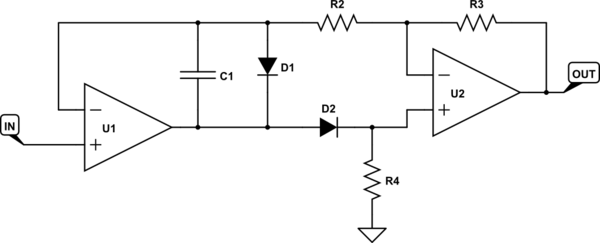
\includegraphics{./img/yYGcS.png}}
 \caption{双电源精密全波整流电路}
 \label{}
\end{figure}

\subsection{方案2:全相位运输阻抗模式精密全波整流电路}

\textbf{原理:} 该设计包括一个完全差分输入和输出的运算放大器,四个二极管,和一个电阻,以实现精密全波整流。

\textbf{优点:}
\begin{itemize}
    \item 精度: 由于运输阻抗模式的设计,可以实现高精度的整流。
    \item 简单的电路结构: 只需要一个运算放大器,四个二极管和一个电阻。
\end{itemize}

\textbf{缺点:} 可能需要特定类型的运算放大器或其他组件,以实现所需的性能。

\begin{figure}[H]
\centering
 \resizebox{0.75\textwidth}{!}{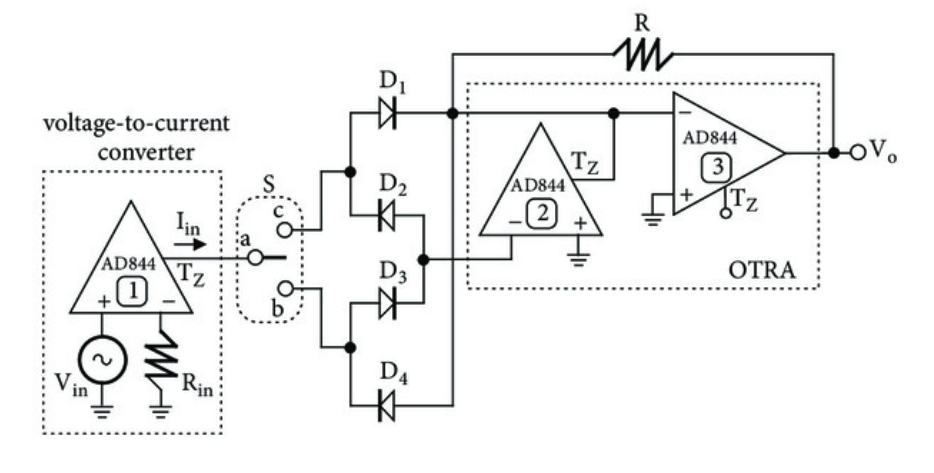
\includegraphics{./img/42.png}}
 \caption{全相位运输阻抗模式精密全波整流电路}
 \label{}
\end{figure}

\subsection{方案3:电压模式精密全波整流电路}

\textbf{原理:} 通过使用包括五个NMOS晶体管的模拟构建块差分电压电流传输放大器(DVCCTA),该方案适用于低电压和高频输入信号。

\textbf{优点:}
\begin{itemize}
    \item 低电压操作: 设计允许在低电压条件下工作。
    \item 高频性能: 适用于高频输入信号的整流。
\end{itemize}

\textbf{缺点:} 电路可能会相对复杂,并且可能需要特定的组件。
\begin{figure}[H]
\centering
 \resizebox{0.75\textwidth}{!}{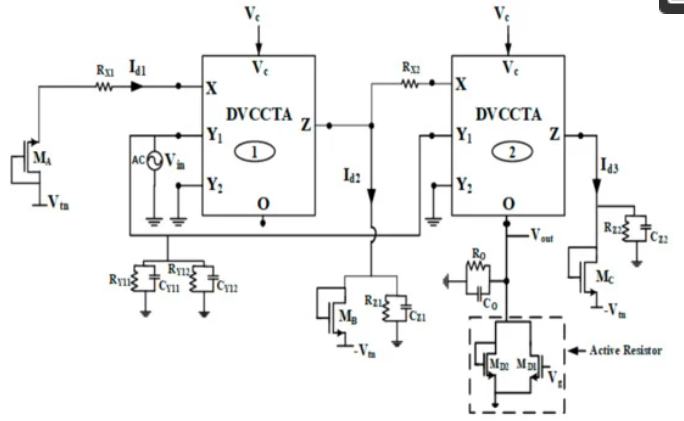
\includegraphics{./img/121450.png}}
 \caption{}
 \label{}
\end{figure}

\subsection{方案4:双绝对值电路设计方案}

\textbf{原理:} 这种设计也称为精密全波整流器(PFWR),它能在两个半周期内产生输出,并且只能在一个方向上产生。它也被称为绝对值电路,因为输出信号的振幅只在正方向上,从而得到输入信号的绝对值\cite{electronics_tutorial}。

\textbf{优点:}
\begin{itemize}
    \item 输出干净: 由于输出信号的振幅只在正方向上,因此能得到干净的输出信号。
    \item 设计简单: 相对于其他方案,这种设计可能更简单,更容易实现。
\end{itemize}

\textbf{选择理由:} 使用双绝对值电路组成双极性精密全波整流电路是所有方案中最为合适的方案,主要基于以下几点考虑:
\begin{itemize}
    \item \textbf{双极性整流能力:} 该方案能够实现双极性整流,处理正负两个电压半周期,使得输出信号能够保持在正向,满足了我们的设计要求。
    \item \textbf{设计和实现的简洁性:} 通过采用双绝对值电路,整个系统的设计和实现变得相对简单和直接,降低了设计难度和实现复杂性。
    \item \textbf{整流精度和信号质量:} 该方案能够保证较高的整流精度和良好的信号质量,满足了精密整流的要求。
    \item \textbf{可扩展性和可调整性:} 具有较好的可扩展性和可调整性,可以通过简单的调整和优化来满足不同的应用需求和性能要求。
    \item \textbf{成本效益:} 与其他方案相比,该方案的成本效益较高,不仅能够满足设计要求,而且在成本和复杂度上都具有一定的优势。
\end{itemize}

最终方案框图如下:

\begin{figure}[H]
\centering
 \resizebox{1\textwidth}{!}{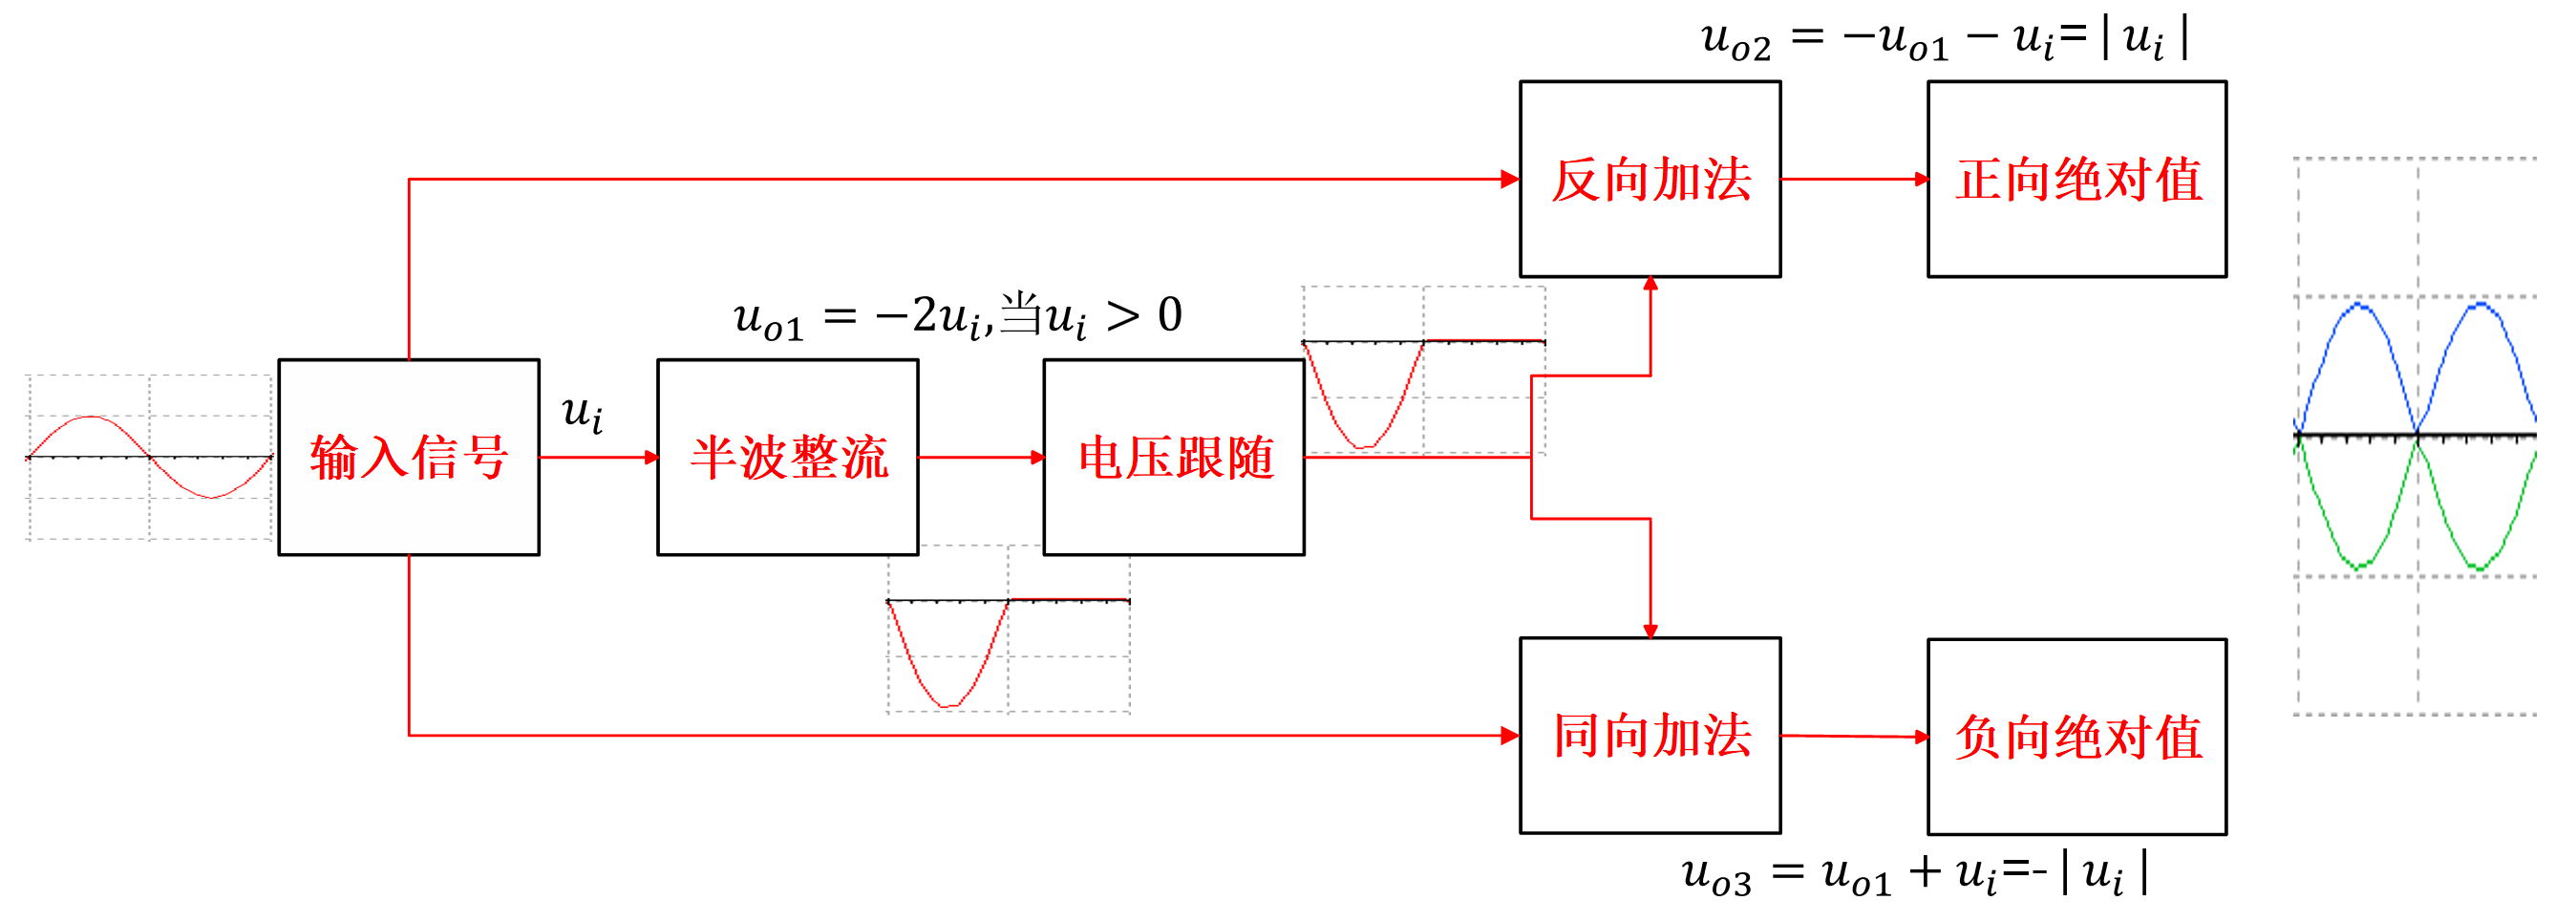
\includegraphics{./img/abs.png}}
 \caption{双绝对值电路方案框图}
 \label{}
\end{figure}

\section{单元电路设计}
\subsection{半波精密整流电路}

半波精密整流电路通常使用运算放大器和两个二极管来实现。它可以提供比传统的半波整流器更好的性能。
\subsubsection{公式推导}

\textbf{当 $u_i > 0$ 时:}

\begin{enumerate}
    \item 输出 \( u_{O1'} \) 为负,因此 \( D_1 \) 截止,而 \( D_2 \) 导通。
    \item 负反馈电流路径为:从 \( u_{O1'} \) 经过 \( D_2 \) 到 \( u_{O1} \),再经过 \( 2R \) 到 \( u_- \)。
    \item 由于运算放大器处于线性工作区,输出 \( u_{O1} \) 为 \( -2u_i \)。
\end{enumerate}

\textbf{当 $u_i < 0$ 时:}

\begin{enumerate}
    \item 输出 \( u_{O1'} \) 为正,因此 \( D_1 \) 导通,而 \( D_2 \) 截止。
    \item 负反馈电流路径为:从 \( u_{O1'} \) 经过 \( D_1 \) 到 \( u_- \)。
    \item 由于 \( D_1 \) 导通,而 \( D_2 \) 截止,\( u_{O1'} \) 约为 \( 0.7V \)(二极管的导通电压)。
    \item 电阻 \( 2R \) 无电流流过,因此 \( u_{O1} \) 为 0。
\end{enumerate}

从以上分析可以看出,只有在 \( u_i > 0 \) 时,输出 \( u_{O1} \) 为非零值,这样就实现了半波整流。当 \( u_i < 0 \) 时,输出 \( u_{O1} \) 为 0,确保了整流的效果。

\subsubsection{元器件选择:}

\begin{itemize}
    \item 运算放大器:LF353D,它具有较低的输入偏置电流和较高的带宽,非常适合此应用。
    \item 二极管:例如 1N4148,这是一个常用的快速开关二极管,适合整流应用。
\end{itemize}

\begin{figure}[H]
\centering
 \resizebox{0.5\textwidth}{!}{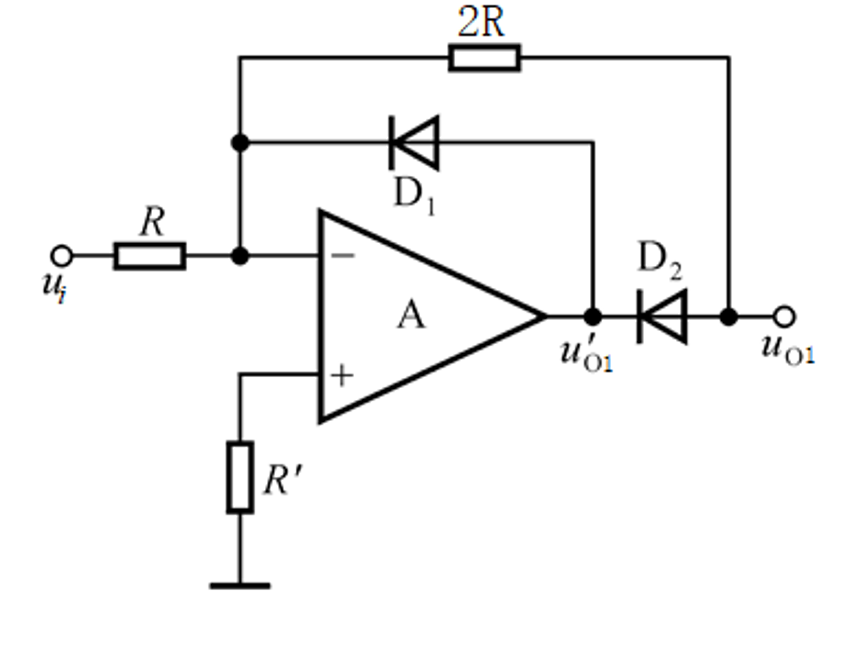
\includegraphics{./img/23457.png}}
 \caption{半波精密整流电路}
 \label{}
\end{figure}

\begin{figure}[H]
\centering
 \resizebox{0.75\textwidth}{!}{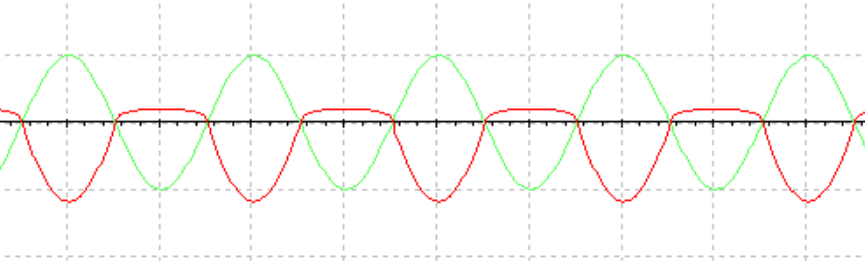
\includegraphics{./img/fz1.png}}
 \caption{半波精密整流电路仿真结果}
 \label{}
\end{figure}
\subsection{电压跟随器}

\subsubsection{设计}
电压跟随器是一种特殊的运算放大器应用,其中运算放大器的输出直接反馈到其反相输入,而信号源直接连接到其非反相输入, 输入电阻高, 输出电阻低,起前后级缓冲作用。

\subsubsection{公式推导}
由于电压跟随器的特性,我们有:
\[ V_{out} = V_{in} \]

\subsubsection{元器件选择}
\begin{itemize}
    \item 运算放大器:LF353D
\end{itemize}

\begin{figure}[H]
\centering
 \resizebox{0.5\textwidth}{!}{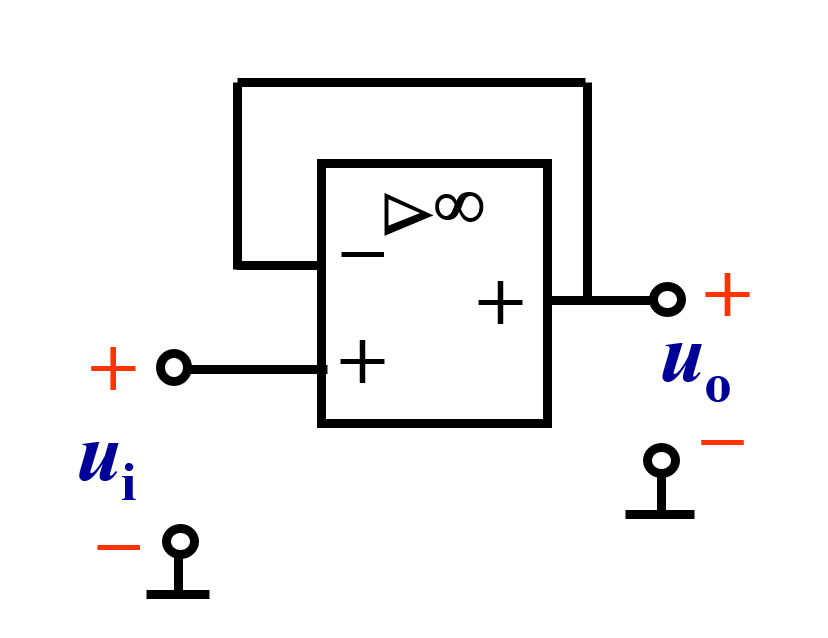
\includegraphics{./img/124400.png}}
 \caption{电压跟随器}
 \label{}
\end{figure}

\subsection{反相加法器}

\subsubsection{设计}
反相加法器的设计涉及多个电阻,并能对多个输入进行加权求和,然后反相输出。

\subsubsection{公式推导}
\[ V_{out} = - \left( \frac{R_f}{R_1} V_{in1} + \frac{R_f}{R_2} V_{in2} + \ldots \right) \]

\subsubsection{元器件选择}
\begin{itemize}
    \item 运算放大器:LF353D
    \item 电阻:根据具体的增益要求选择
\end{itemize}
\begin{figure}[H]
\centering
 \resizebox{0.5\textwidth}{!}{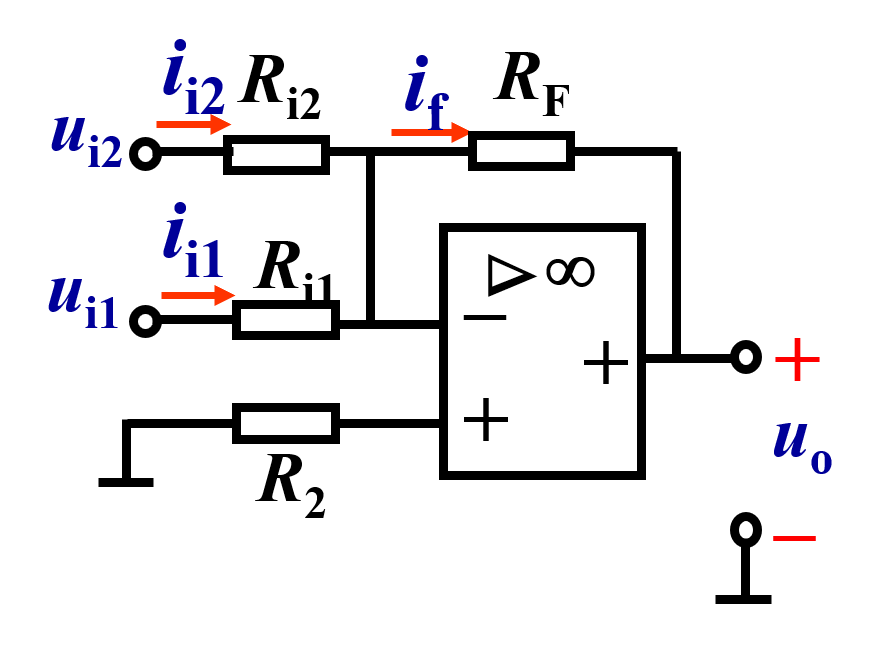
\includegraphics{./img/124744.png}}
 \caption{反相加法器}
 \label{}
\end{figure}
\subsection{同相加法器}

\subsubsection{设计}
同相加法器可以对多个输入进行加权求和,然后输出。

\subsubsection{公式推导}
\[ V_{out} = \left( 1 + \frac{R_f}{R_1} \right) V_{in1} + \left( 1 + \frac{R_f}{R_2} \right) V_{in2} + \ldots \]

\subsubsection{元器件选择}
\begin{itemize}
    \item 运算放大器:LF353D
    \item 电阻:根据具体的增益要求选择
\end{itemize}
\begin{figure}[H]
\centering
 \resizebox{0.5\textwidth}{!}{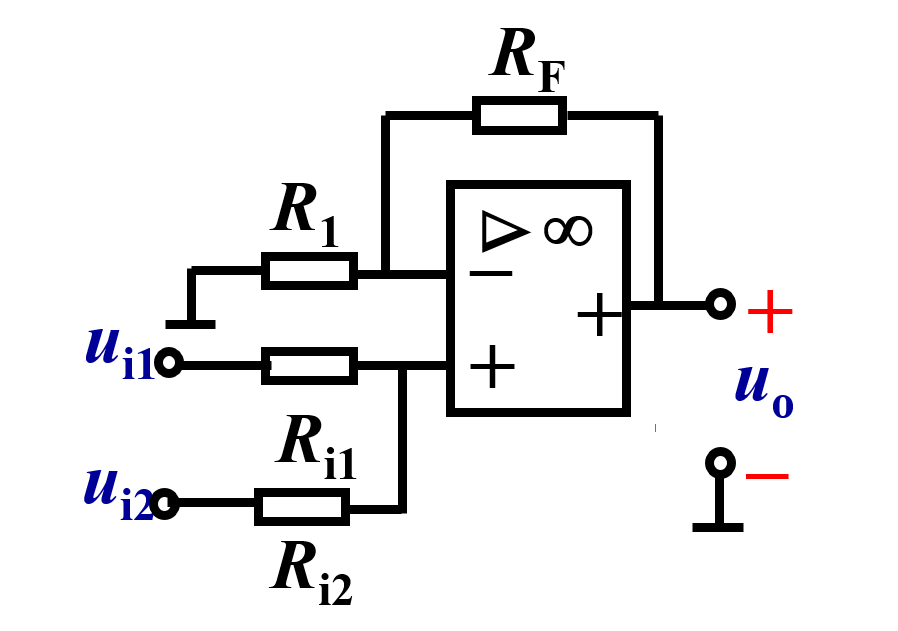
\includegraphics{./img/124937.png}}
 \caption{同相加法器}
 \label{}
\end{figure}

\section{电路整体设计}
整体电路设计如下图所示:
\begin{figure}[H]
\centering
 \resizebox{0.75\textwidth}{!}{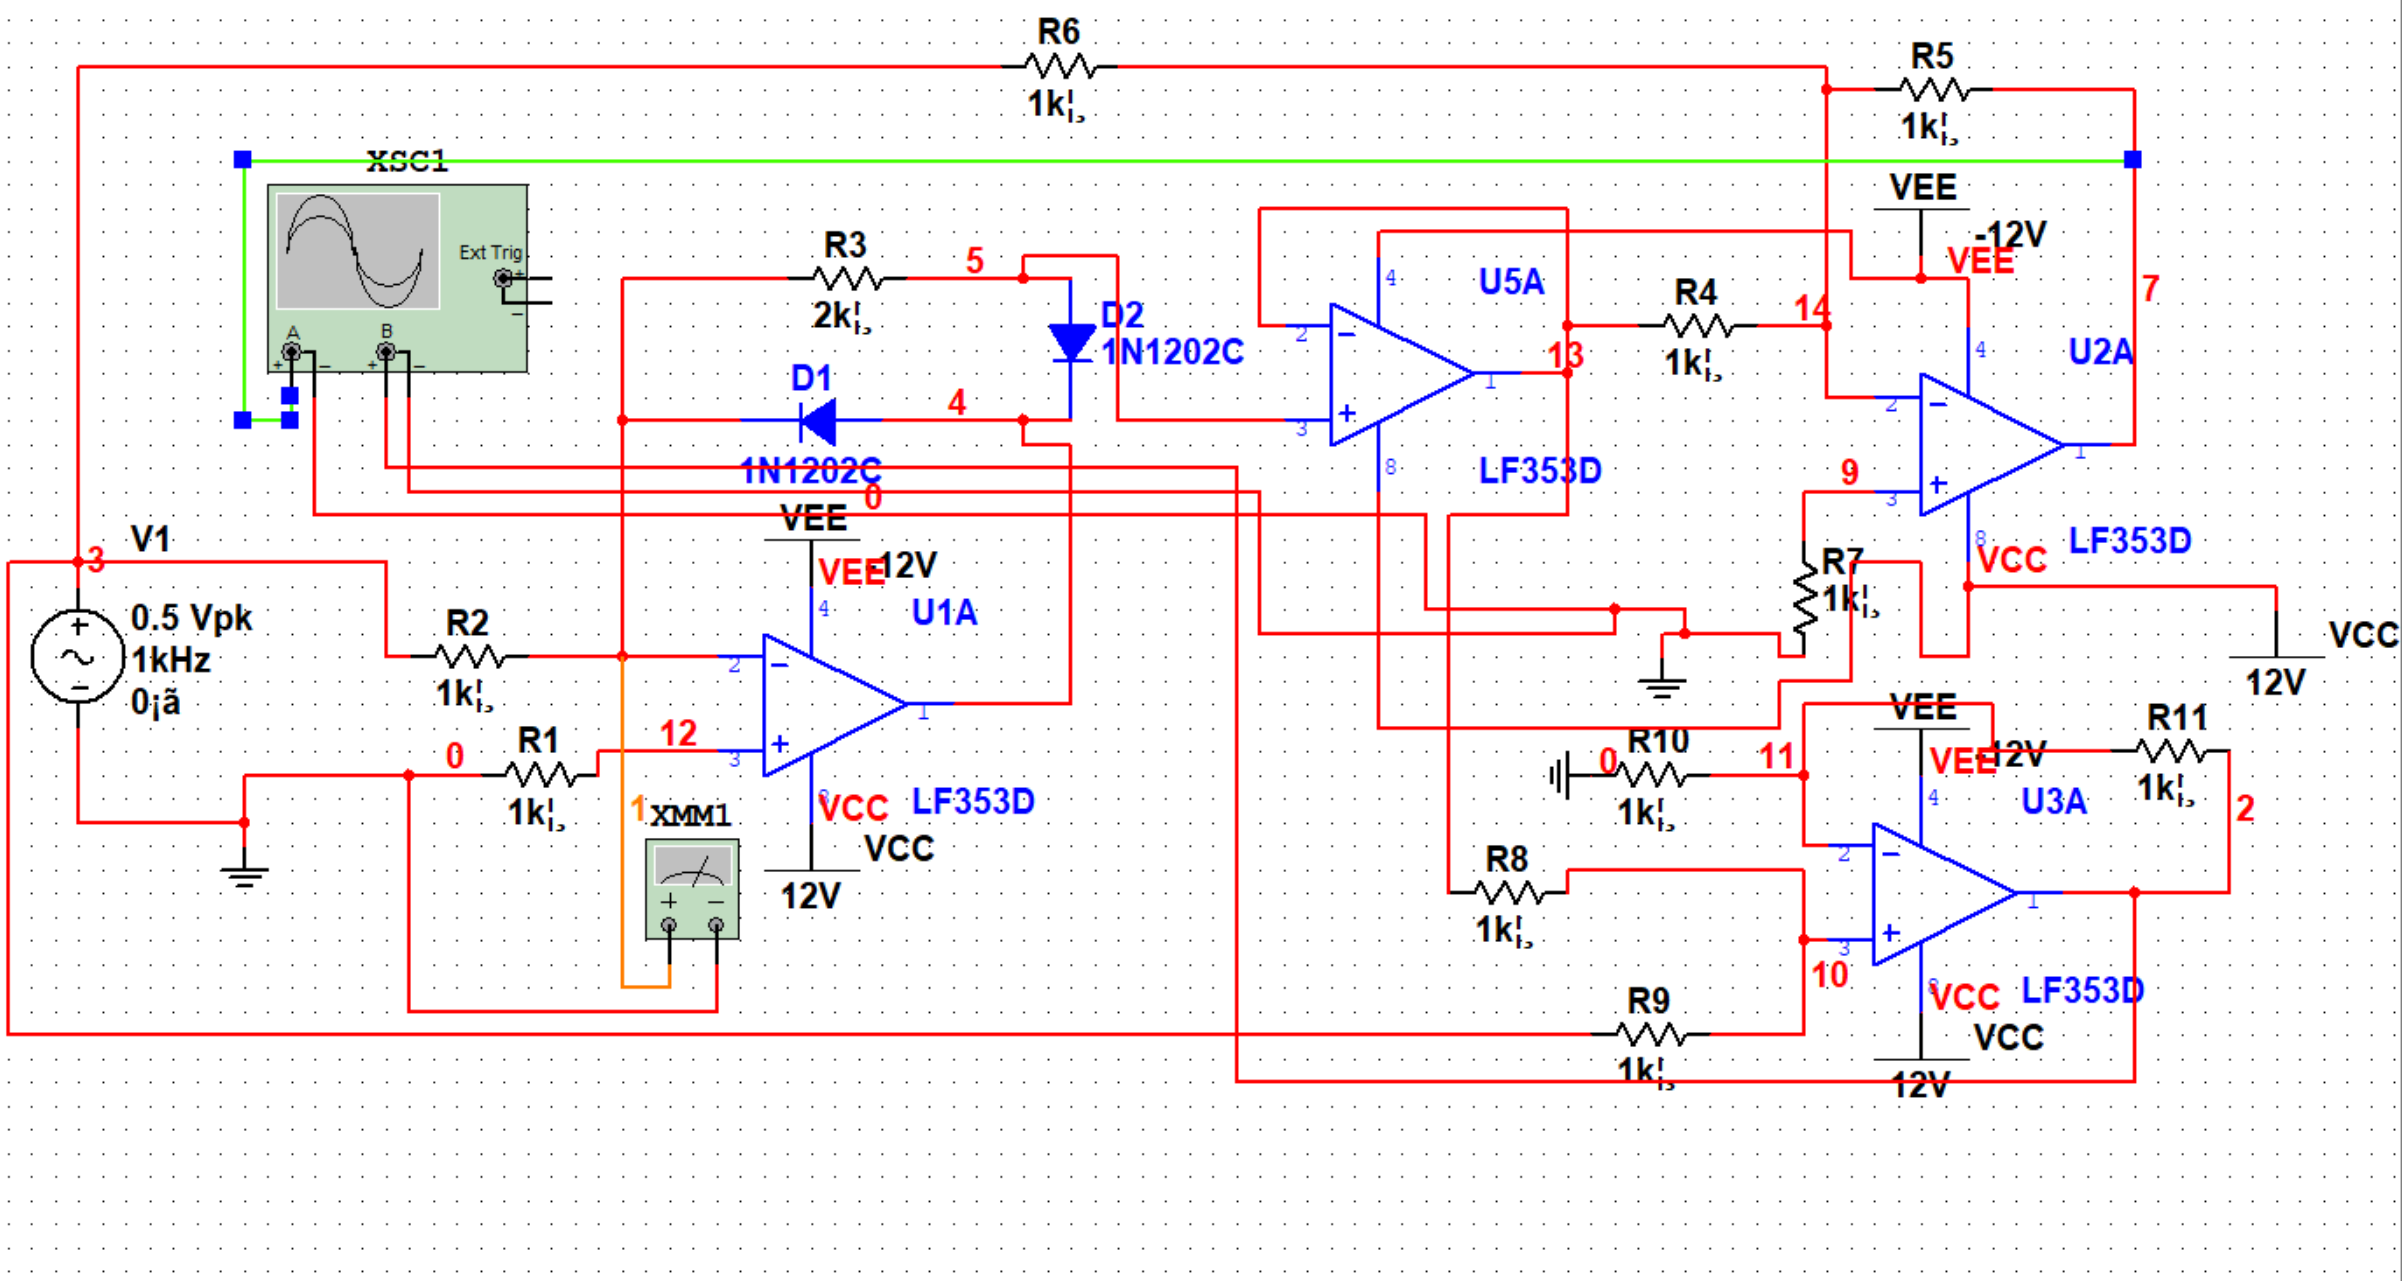
\includegraphics{./img/125338.png}}
 \caption{电路整体设计}
 \label{}
\end{figure}

电路工作原理如下:
\begin{itemize}
    \item \textbf{输入信号}:在本场景中,输入为一个幅值为500mVpk、频率为1kHz的正弦波信号。这代表了我们需要处理的原始信号。
    
    \item \textbf{半波精密整流}:
    \begin{itemize}
        \item 整流电路的核心是一个二极管(D1)和一个运放。
        \item 当输入信号为正时,D1导通,信号得以通过;当输入为负时,D1截止,信号被阻断。
        \item 由于运放和电阻的影响,输出信号幅值为-979mV。
    \end{itemize}
    \begin{figure}[H]
        \centering
         \resizebox{0.75\textwidth}{!}{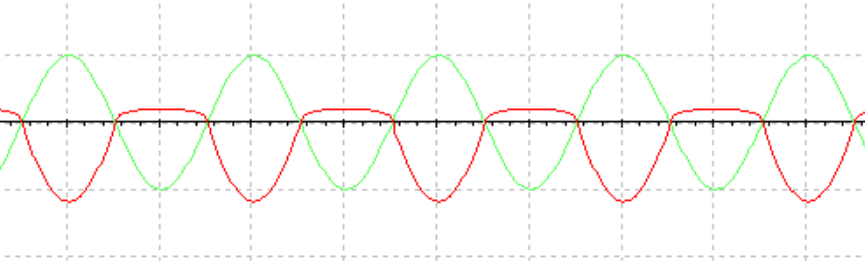
\includegraphics{./img/fz1.png}}
         \caption{半波精密整流电路仿真结果}
         \label{}
        \end{figure}
    \item \textbf{电压跟随器}:电压跟随器是一个特殊的运放应用,确保输出信号完美跟随输入,输出信号的幅值保持为-979mV。
    \begin{figure}[H]
        \centering
         \resizebox{0.75\textwidth}{!}{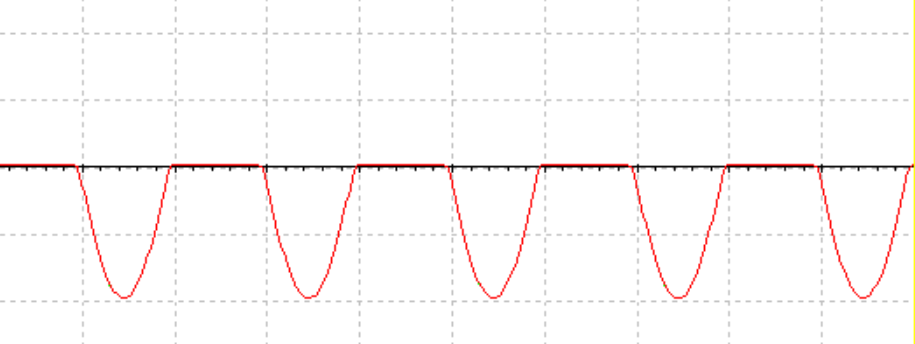
\includegraphics{./img/fz2.png}}
         \caption{电压跟随器仿真结果}
         \label{}
        \end{figure}
    \item \textbf{反向加法器}:
    \begin{itemize}
        \item 这个电路接收-979mV的信号,并将其反相。
        \item 同时,它还接收了一个500mV的正偏置信号。
        \item 最终得到478mV的正半波信号。
    \end{itemize}
    \begin{figure}[H]
        \centering
         \resizebox{0.75\textwidth}{!}{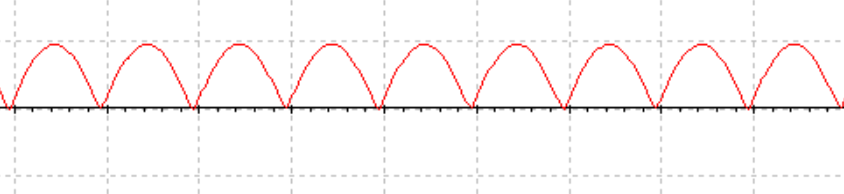
\includegraphics{./img/fz3.png}}
         \caption{反向加法器仿真结果}
         \label{}
        \end{figure}

    \item \textbf{同向加法器}:
    \begin{itemize}
        \item 与反向加法器不同,同向加法器不会反相信号。
        \item 它直接将-979mV的信号与500mV的信号相加。
        \item 最终得到-478mV的负半波信号。
    \end{itemize}
    \begin{figure}[H]
        \centering
         \resizebox{0.75\textwidth}{!}{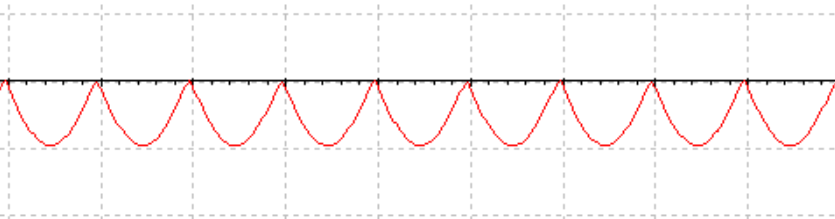
\includegraphics{./img/fz4.png}}
         \caption{同向加法器仿真结果}
         \label{}
        \end{figure}
    \item \textbf{输出信号}:经过上述处理,最终得到两个半波信号:一个478mV的正半波和一个-478mV的负半波。这两个信号加在一起,形成了一个完整的双极性信号。
    \item \begin{figure}[H]
        \centering
         \resizebox{0.75\textwidth}{!}{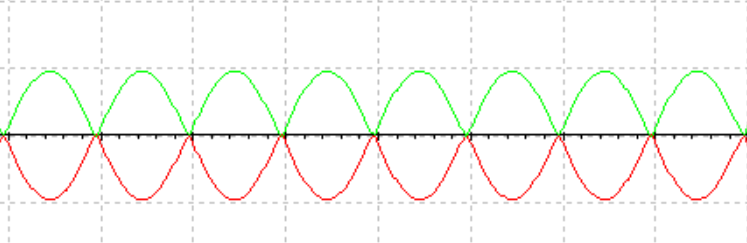
\includegraphics{./img/fz5.png}}
         \caption{最终输出}
         \label{}
        \end{figure}
\end{itemize}
\bibliographystyle{plain}
\bibliography{references}
\end{document}